\section{Partial Derivatives}
\subsection{Surfaces and Graphs}\hypertarget{surf1}
In parametric curves, we considered parametric functions in 2 and 3-dimensional space, where a 1 dimensional input yields a multi-dimensional vector output. Next, we'll consider what happens when we use a multidimensional input to give a single output. Where parametric curves were often coded as projectile motion, there are a vast amount of models that take multiple inputs. Of particular interest to us will be multivariate optimization, which mirrors the constrained optimization problems from Calculus II. Lets get to some formality: as we're working in 3-d space mostly in this class, we'll mostly consider functions with a two dimensional input (usually $(x,y)$) and a one dimensional output (usually $z$).

\begin{definition}{Graphs of Surfaces}
Let $f$ be a function, $f:\bbr^2\to\bbr$. Then the graph of $f$ is the set of points $$\big\{\big(x,y,f(x,y)\big)\ : \ (x,y)\in \bbr^2 \big\}.$$ This graph appears as a surface in $3$-d space when graphed with the output along the $z$-axis. We often write $z=f(x,y)$ as a shorthand for this surface (this parallels the convention where we write $y=f(x)$ in 2-space).
\end{definition}

\begin{example}{A Surface}
Consider the function $f(x,y)=10-x^2+y^3-3y^2-6y$. The graph of this surface looks like this:
\vspace{1em}
\begin{center}
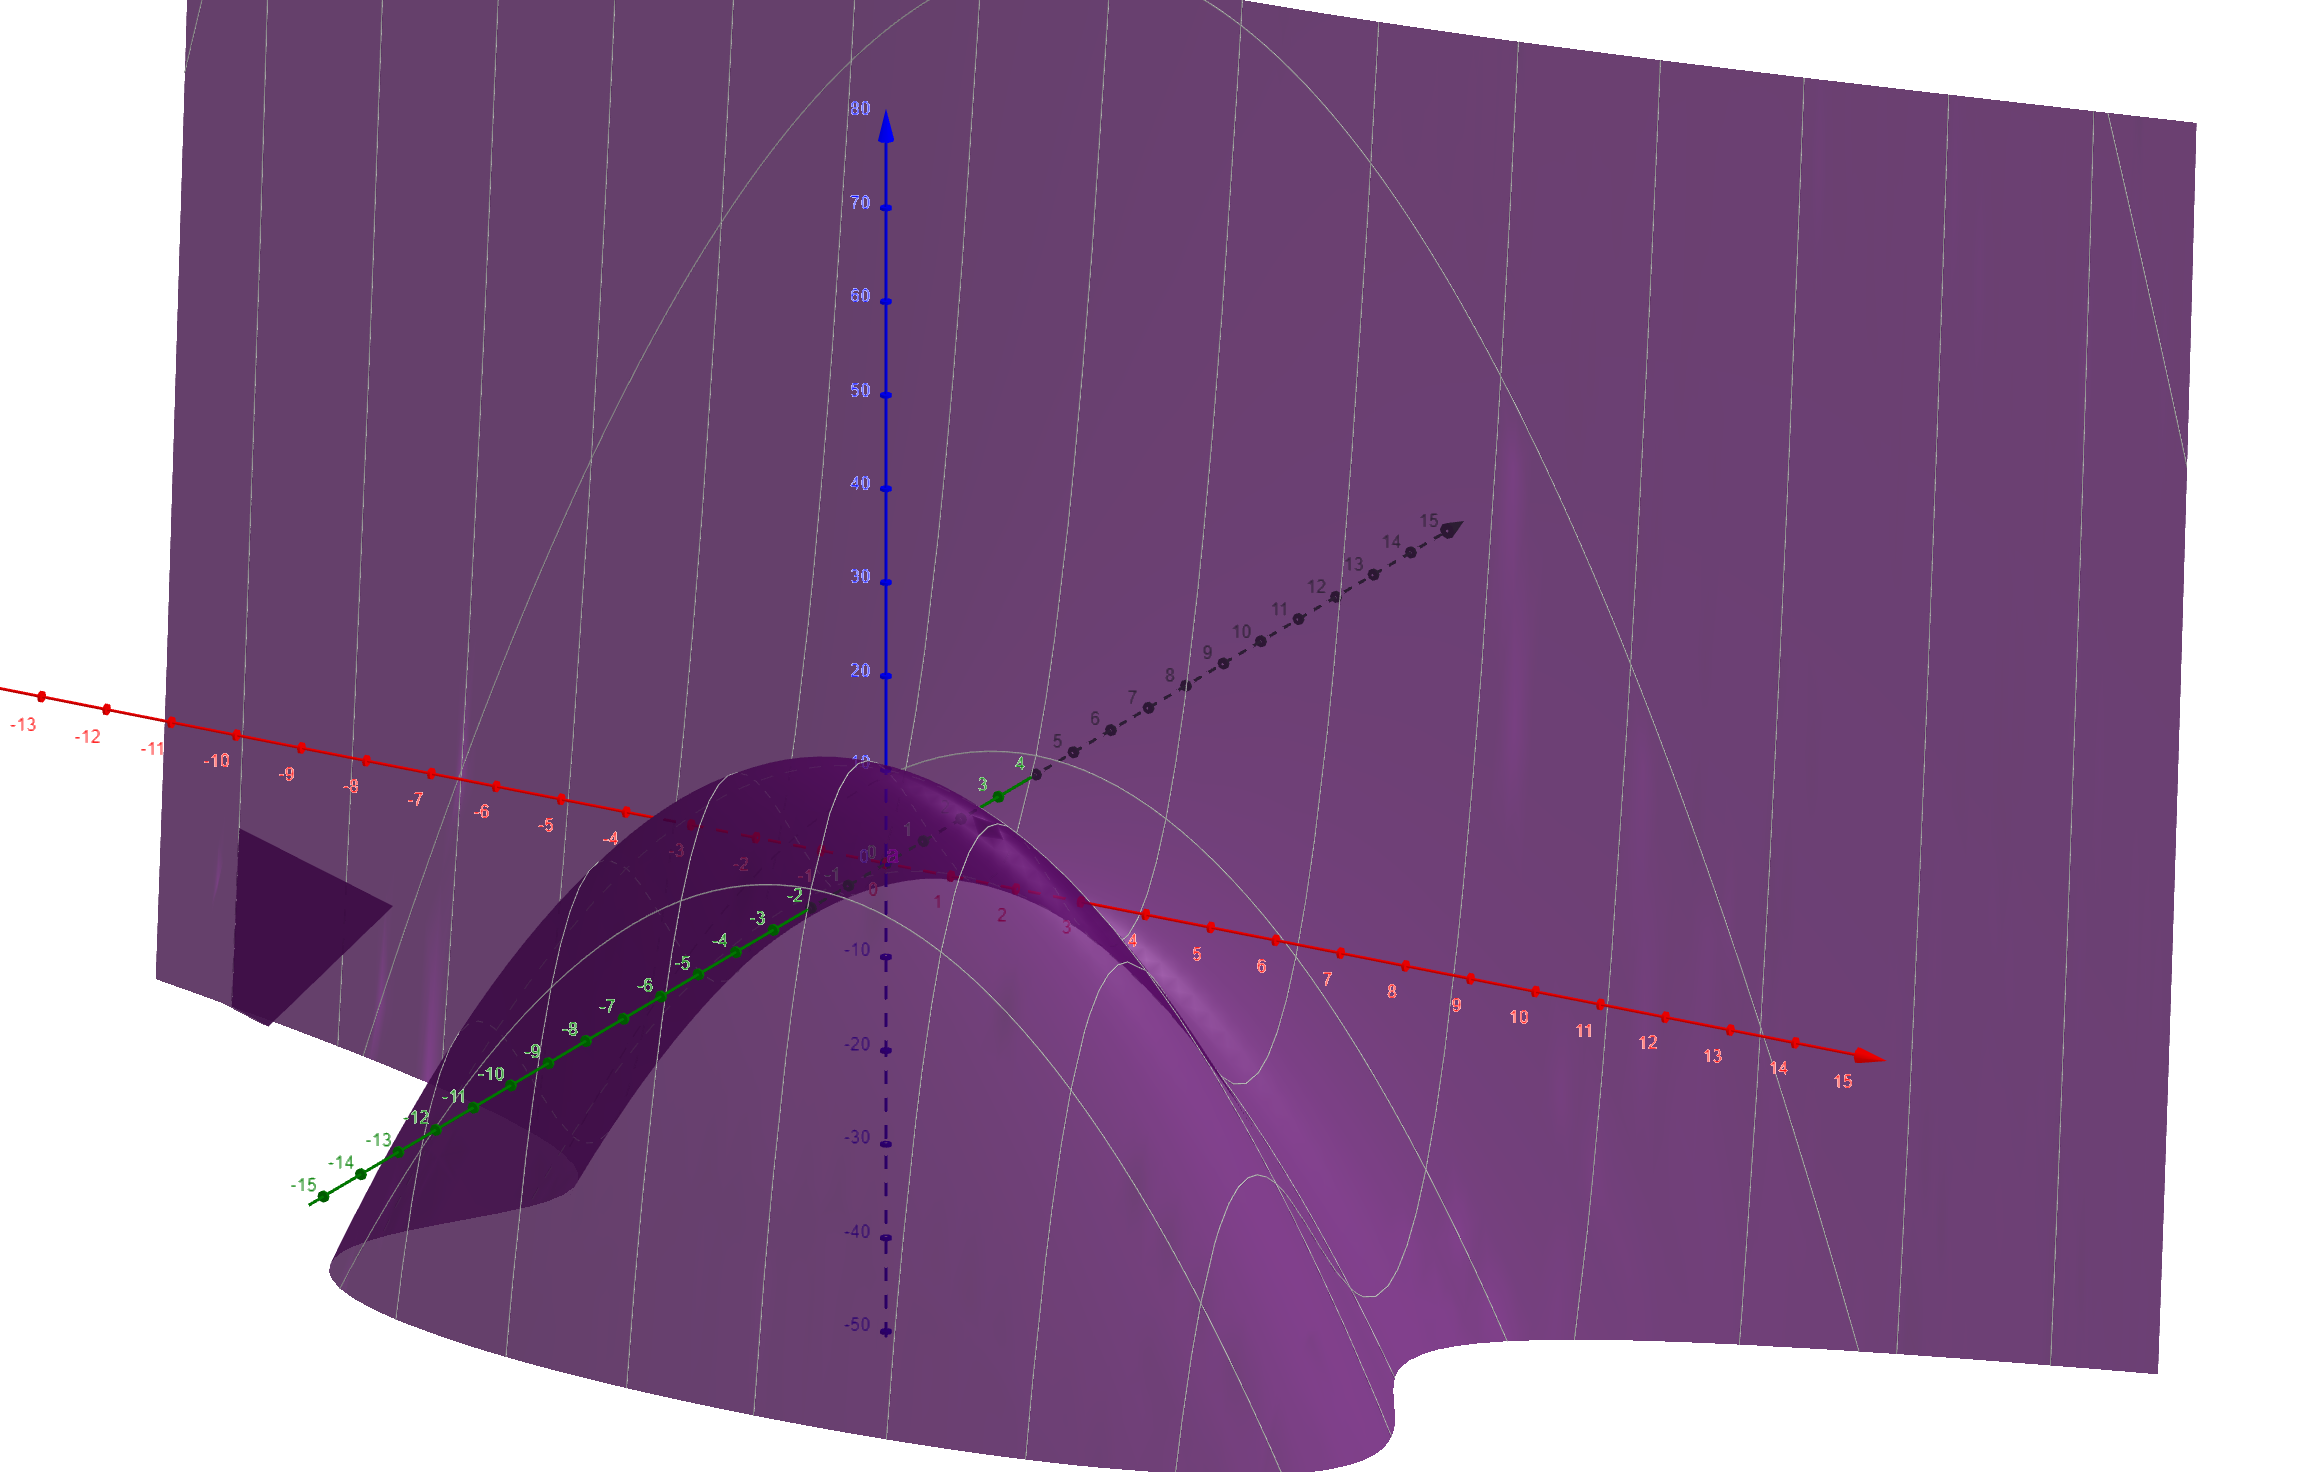
\includegraphics[scale=0.2]{Figures/surfaceex1} \\
 \href{https://www.geogebra.org/3d/gzy3xxgh}{Geogebra Link to Graph}
\end{center}
\end{example}

Visualizing 3-dimensional surfaces in 2-dimensional space can be a little tricky. We can, of course, use clever perspective, and Geogebra 3d lets us rotate the object and get a very good sense of it. Another useful technique is the \textbf{contour plot}. A common application of contour plots is topographic maps, where a contour plot is used to display elevation changes.

\begin{center}
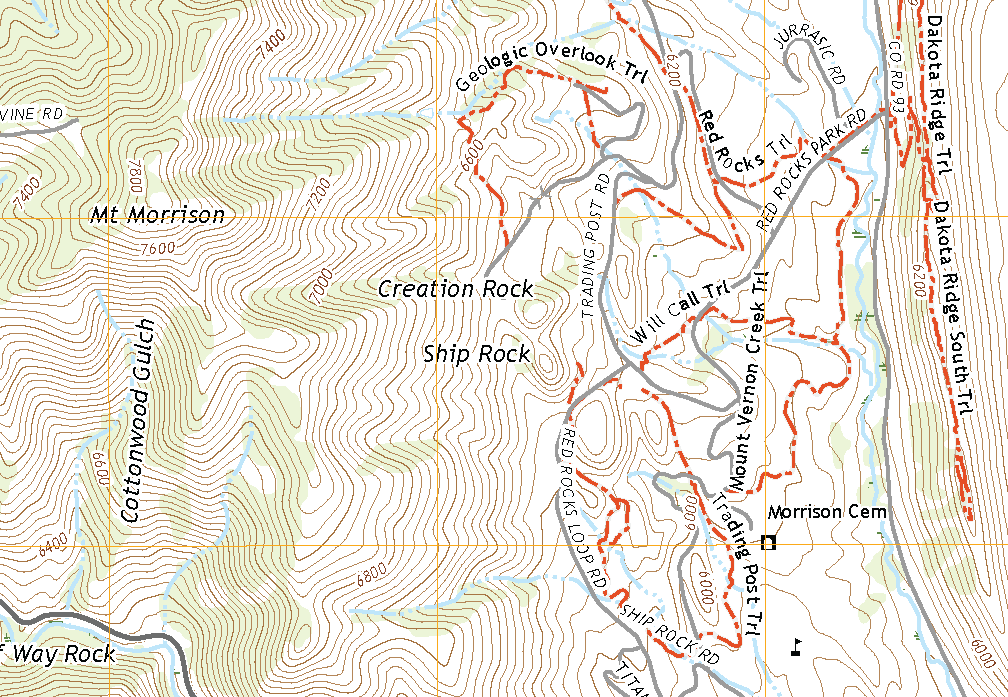
\includegraphics[scale=0.48]{Figures/redrocks}\\
Topographic Map of the area around Red Rocks in Morrison, Colorado.
\end{center}

A contour plot of a surface consists of a set of \textbf{level curves}, each of which are the intersection of the surface $f(x,y)=z$ and the plane $z=c$ for some $c\in\bbr$. That is, they are the collection of $2$-dimensional graphs, $f(x,y)=c$.

\begin{example}{Level Curves and Contour Plots}
Consider the same function as before, $f(x,y)=10-x^2+y^3-3y^2-6y$. We construct the following level curves:
\begin{align*}
-6=&10-x^2+y^3-3y^2-6y\\
-3=&10-x^2+y^3-3y^2-6y\\
0=&10-x^2+y^3-3y^2-6y\\
3=&10-x^2+y^3-3y^2-6y\\
6=&10-x^2+y^3-3y^2-6y\\
9=&10-x^2+y^3-3y^2-6y\\
12=&10-x^2+y^3-3y^2-6y.
\end{align*}
This yields the following contour plot:
\vspace{1em}
\begin{center}
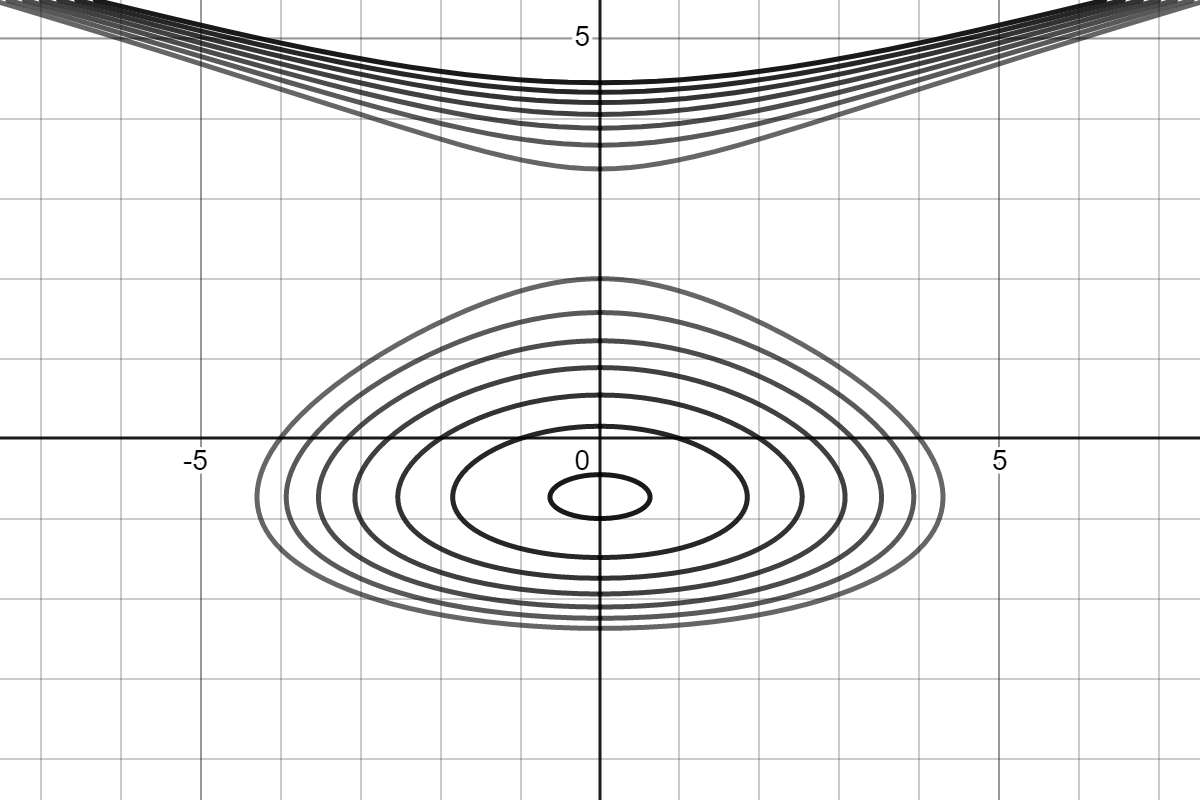
\includegraphics[scale=0.3]{Figures/contourex1}\\
Contour plot of $f(x,y)=10-x^2+y^3-3y^2-6y$.
\end{center}
\end{example}

\begin{exercise}{Level Curves}
\begin{enumerate}
\item Consider the function $f(x,y)=\sqrt{16-x^2-y^2}$. (don't graph this on geogebra yet!) Construct a set of level curves where $z=0$, $z=1$, $z=2$, $z=3$ and $z=4$, then produce a contour plot. Hint: You should be able to graph these without a computer graphing tool. Try squaring both sides of the level curve equation then rewriting it in the form $x^2+y^2=r^2$, which is a circle with radius $r$. 
\vspace{1em}
\item Can you conjecture what the graph of the surface looks like? Check your conjecture using Geogebra 3d.
\end{enumerate}
\end{exercise}
